% Copyright (C) 2012 Davidlohr Bueso <dave@gnu.org>

% API STUFF
\section{New Internal API}
\begin{frame}\frametitle{New Internal API}
  \begin{itemize}
  \item Create an abstraction level between fdisk-family tools and lower-level disklabel logic.
  \item Use a driver based model to deal with disklabels and handle \emph{events} through callbacks.
  \item The API can be seen as:
    \begin{enumerate}
    \item handle generic disk logic (like disk topology, sectors, MBR)
    \item gateway for disklabel specific demads (like probing or deleting a partition).
    \end{enumerate}
  \item Everything fdisk is capable of doing is goverened by a \textbf{fdisk context}.
  \item API users need not worry about internals.
  \end{itemize}
\end{frame}

\subsection{Architectural Overview}
\begin{frame}
  \center{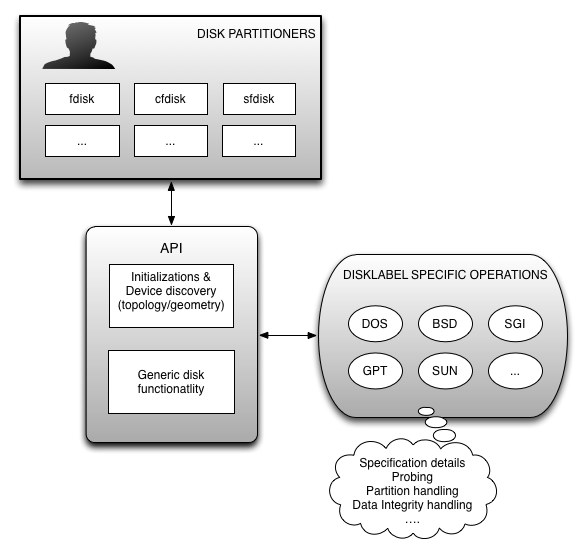
\includegraphics[scale=0.5]{img/fdisk-arch.png}}
\end{frame}

\subsection{API Benefits}
\begin{frame}\frametitle{API Benefits}
  \begin{itemize}
  \item Unifies concepts and specifications behind different partition formats.
  \item Simplifies dealing with disklabel specifics.
  \item Makes the code easier to read and modify.
  \item Makes detecting existing bugs easier and reduces the probability of introducing new bugs.
  \item Once complete, the idea is to create a shared library - similar to what libparted is to GNU parted.
  \end{itemize}
\end{frame}
